\documentclass{report} 
\usepackage{graphicx}
\usepackage{amsmath}
\usepackage{float}
\usepackage{titlesec}
\usepackage{subcaption}
\usepackage{caption}

% Number figures as <chapter>.<section>.<figure>
\renewcommand\thefigure{\thechapter.\thesection.\arabic{figure}}
\counterwithin{figure}{section}

\titlelabel{\thetitle.\quad}

\setlength{\parskip}{1em}
\setlength{\parindent}{0pt}
\begin{document}

\setcounter{chapter}{4}  % Start from chapter 6
\section*{Chapter 4:  Respiratory Sound Classification}



\section*{Introduction}
This section outlines the complete data mining workflow used to develop the respiratory sound classification system, following the CRISP-DM (Cross-Industry Standard Process for Data Mining) methodology. Each sub-section corresponds to a phase in the CRISP-DM cycle—from business understanding and data acquisition to modeling, evaluation, and deployment. Particular emphasis is placed on handling multimodal data, where audio recordings of lung sounds are complemented by metadata extracted from clinical PDF reports. The use of CLAP (Contrastive Language-Audio Pretraining) enables effective fusion of these modalities for downstream classification. This structured approach ensures the development is methodical, clinically relevant, and technically robust.

\newpage
\section{Business Understanding} 
\subsection{Business Objectives}
This project aims to classify respiratory conditions by leveraging multimodal data — specifically, lung auscultation audio and patient metadata (e.g., symptoms, notes). To accomplish this, we employ the CLAP \cite{hsu2023clap}  (Contrastive Language-Audio Pretraining) architecture to embed both modalities into a shared latent space. These joint embeddings are then passed to a lightweight classifier to predict respiratory sound categories such as \textit{normal}, \textit{wheeze}, or \textit{crackle}.

This approach supports healthcare professionals by:
\begin{itemize}
    \item Enhancing diagnostic accuracy using combined audio-text context.
    \item Reducing time and subjectivity in manual auscultation interpretation.
    \item Providing AI-driven assistance in remote or resource-limited healthcare settings.
\end{itemize}

Stakeholders include:
\begin{itemize}
    \item \textbf{Clinicians:} Benefit from real-time AI-supported diagnostics.
    \item \textbf{Patients:} Gain earlier and more accurate diagnoses.
    \item \textbf{Medical Device Manufacturers:} Can integrate the classifier into stethoscope hardware.
    \item \textbf{Regulatory Authorities:} Ensure compliance and certification for clinical deployment.
    \item \textbf{Research and Development Teams:} Responsible for system design and performance.
\end{itemize}

\subsection{Project Goals}
\begin{itemize}
    \item Use CLAP to generate multimodal embeddings from respiratory audio and patient text descriptions.
    \item Train a high-performing classifier on these embeddings to predict diagnostic categories.
    \item Ensure clinical interpretability and real-time deployment readiness.
\end{itemize}

\subsection{Constraints and Risks}
\begin{itemize}
    \item \textbf{Data Privacy:} Must comply with HIPAA/GDPR when processing patient metadata.
    \item \textbf{Multimodal Alignment:} Embeddings from CLAP must capture relevant diagnostic features from both audio and text.
    \item \textbf{Generalization:} Risk of underfitting due to class imbalances between the labels "wheeze" , "crackles" , "normal" , "both".
    \item \textbf{Clinical Interpretability:} Must justify predictions for clinician trust and regulatory approval.
\end{itemize}

\subsection*{Summary}
This project proposes a novel application of CLAP for multimodal fusion in respiratory sound classification. By embedding both patient audio and textual information into a shared space and using a downstream classifier, the system enables accurate, fast, and explainable predictions. Success depends on a robust technical pipeline, regulatory alignment, and demonstrated clinical utility.


\section*{4.2 Data Understanding}

\paragraph{4.2.1 Data Sources \\}
The primary dataset used for training the model is the \textbf{ICBHI 2017 Respiratory Sound Database}, which includes:
\begin{itemize}
    \item \textbf{Audio recordings} of lung sounds collected from 126 patients using an electronic stethoscope.
    \item \textbf{Metadata files}, such as demographic information and clinical diagnoses.
    \item \textbf{Segmentation annotations} indicating labeled intervals of respiratory events (inspiration, expiration).
\end{itemize}

\paragraph{4.2.2 Loaded Data\\}
Three key components were extracted:
\begin{enumerate}
    \item \textbf{Diagnosis Labels:} A CSV file (\texttt{patient\_diagnosis.csv}) mapping patient IDs to their respiratory condition (e.g., asthma, COPD, pneumonia).
    \item \textbf{Demographic Metadata:} A text file containing age, sex, BMI, and child-specific attributes like height and weight.
    \item \textbf{Audio Files:} Multiple WAV files per patient, capturing respiratory cycles in varying environments and conditions.
\end{enumerate}

\paragraph{4.2.3 Exploratory Analysis\\}
The following steps were conducted to better understand the data:
\begin{itemize}
    \item Inspected class distribution to identify imbalance (e.g., overrepresentation of "healthy" vs. "COPD").
    \item Visualized audio signal characteristics such as waveform length, sampling rate consistency, and signal-to-noise ratio.
    \item Merged demographic and diagnosis data by patient ID to facilitate multimodal embedding.
    \item Generated descriptive sentences per patient from structured metadata, such as:
    \textit{"Patient 101 is a 65-year-old male. The adult has a BMI of 27.3 kg/m²."}
\end{itemize}

\paragraph{4.2.4 Challenges Identified\\}
\begin{itemize}
    \item \textbf{Missing Data:} Some entries lack age, BMI, or diagnosis labels, requiring filtering or imputation.
    \item \textbf{Class Imbalance:} Certain respiratory conditions are underrepresented, potentially biasing the classifier.
    \item \textbf{Variable Audio Lengths:} Recording durations vary significantly, requiring padding or trimming during preprocessing.
    \item \textbf{Data Heterogeneity:} Audio captured in uncontrolled environments introduces noise and inconsistency.
\end{itemize}

\paragraph{Summary \\}
The dataset provides a rich combination of audio and clinical metadata, which is essential for multimodal learning. By using CLAP to embed both the auscultation sounds and textual descriptions, the project exploits this diversity to improve classification performance. A thorough understanding of the dataset’s structure and limitations guided preprocessing and model design choices.


\section{Data Preparation}

\subsection*{Overview}
To enable the use of the CLAP (Contrastive Language-Audio Pretraining) model, both audio signals and textual descriptions were preprocessed and aligned into a format suitable for joint embedding. Data preparation involved several key stages: cleaning, transformation, feature generation, and multimodal input construction.

\subsection{Audio Preprocessing}
\begin{itemize}
    \item \textbf{Loading:} WAV audio files were loaded using \texttt{torchaudio} with consistent settings across all samples.
    \item \textbf{Resampling:} All audio signals were resampled to 48\,kHz to match the input requirements of the CLAP model.
    \item \textbf{Normalization:} Amplitude normalization was applied to reduce variability in recording loudness.
    \item \textbf{Device Filtering:} Only audio recorded using a microphone device was retained; recordings captured via stethoscope or user-recorded samples were excluded to ensure consistency and realistic ambient conditions.
\end{itemize}

\subsection{Text Preprocessing}
\begin{itemize}
    \item \textbf{Demographic Metadata Integration:} Patient age, sex, and physical metrics were combined into a coherent textual description.
    \item \textbf{Description Generation:} A custom function generated natural language sentences, e.g., \textit{"Patient 103 is a 7-year-old female child weighing 22 kg and measuring 120 cm in height."}
    \item \textbf{Tokenization:} Descriptions were tokenized using the CLAP processor to match the format of its language encoder.
    \item \textbf{Missing Value Handling:} Patients missing critical metadata fields were assigned defaults.
\end{itemize}

\subsection{Multimodal Pair Construction}
Each input sample consisted of a synchronized multimodal pair:
\begin{enumerate}
    \item A preprocessed 5-second audio tensor representing a single breathing cycle.
    \item A text description specific to the patient from whom the audio was collected.
\end{enumerate}
These were fed into the CLAP model to generate aligned audio-text embeddings in a shared latent space.

\subsection{Label Encoding}
\begin{itemize}
    \item Respiratory condition labels (e.g., crackles, wheezes, normal) were derived from expert annotations per breathing cycle.
    \item Labels were encoded using \texttt{LabelEncoder} from \texttt{scikit-learn} to obtain numerical class indices.
    \item Ambiguous or unlabeled cycles were excluded to avoid introducing noise in the training process.
\end{itemize}

\subsection{Dataset Splitting}
\begin{itemize}
    \item An official dataset split provided by the dataset curators was used to separate training and test sets.
    \item This ensured reproducibility and comparability with prior work.
    \item Patient-level disjointness was maintained: no subject appeared in both training and test sets, preventing data leakage.
\end{itemize}

\subsection*{Summary}
The preprocessing pipeline standardized and aligned audio and text inputs for CLAP-based embedding. Filtering by recording device, adherence to the official train/test split, and careful label and segmentation handling ensured high-quality inputs for downstream classification.

\section*{4.4 Environment and Libraries}

\paragraph{4.4.1 Hardware and Platform\\}
All experiments and training were conducted using Kaggle Notebooks, which offer a reliable, GPU-accelerated, cloud-based development environment. The specific hardware configuration was:

\begin{itemize}
    \item \textbf{Platform:} Kaggle Notebooks
    \item \textbf{GPU:} NVIDIA Tesla T4 (16 GB VRAM)
    \item \textbf{CPU:} Dual-core virtual CPU (provided by Kaggle)
    \item \textbf{Memory:} Approximately 13–16 GB RAM
    \item \textbf{Operating System:} Ubuntu-based container
\end{itemize}

\paragraph{4.4.2 Programming Language\\}
The implementation was carried out in \textbf{Python 3.10}, chosen for its strong ecosystem in machine learning and scientific computing.

\paragraph{4.4.3 Key Libraries and Frameworks\\}
A variety of libraries and tools were used to support different stages of the pipeline:

\begin{itemize}
    \item \textbf{PyTorch:} Core framework for deep learning and model development.
    \item \textbf{torchaudio:} For loading and preprocessing waveform audio.
    \item \textbf{transformers (Hugging Face):} Used for CLAP’s audio and text encoders and tokenization.
    \item \textbf{scikit-learn:} Utility functions for stratified splitting, label encoding, and evaluation.
    \item \textbf{pandas \& numpy:} For data manipulation, transformation, and numerical operations.
    \item \textbf{matplotlib \& seaborn:} Visualization of confusion matrices and performance metrics.
    \item \textbf{os \& glob:} Used for file traversal and organizing input data.
\end{itemize}

\paragraph{4.4.4 Reproducibility\\}
To ensure consistent and reliable results:
\begin{itemize}
    \item Random seeds were set across NumPy and PyTorch.
    \item The official train/test split provided with the dataset was used.
    \item All key hyperparameters (e.g., learning rate, weight decay, batch size) were fixed and reused.
\end{itemize}

\paragraph{Summary\\}
The CLAP-based multimodal classification model was trained and validated using Kaggle's GPU-enabled environment. Open-source libraries provided the foundation for efficient model development, training, and evaluation in a fully reproducible pipeline.

\break
\section{Modeling}

\paragraph{Overview}
The core modeling strategy involves using the CLAP (Contrastive Language-Audio Pretraining) model to transform heterogeneous input data — audio signals and textual patient metadata — into a unified latent representation. These embeddings are then passed through a custom multi-layer neural network for classification.

\begin{figure}[H]
    \centering
    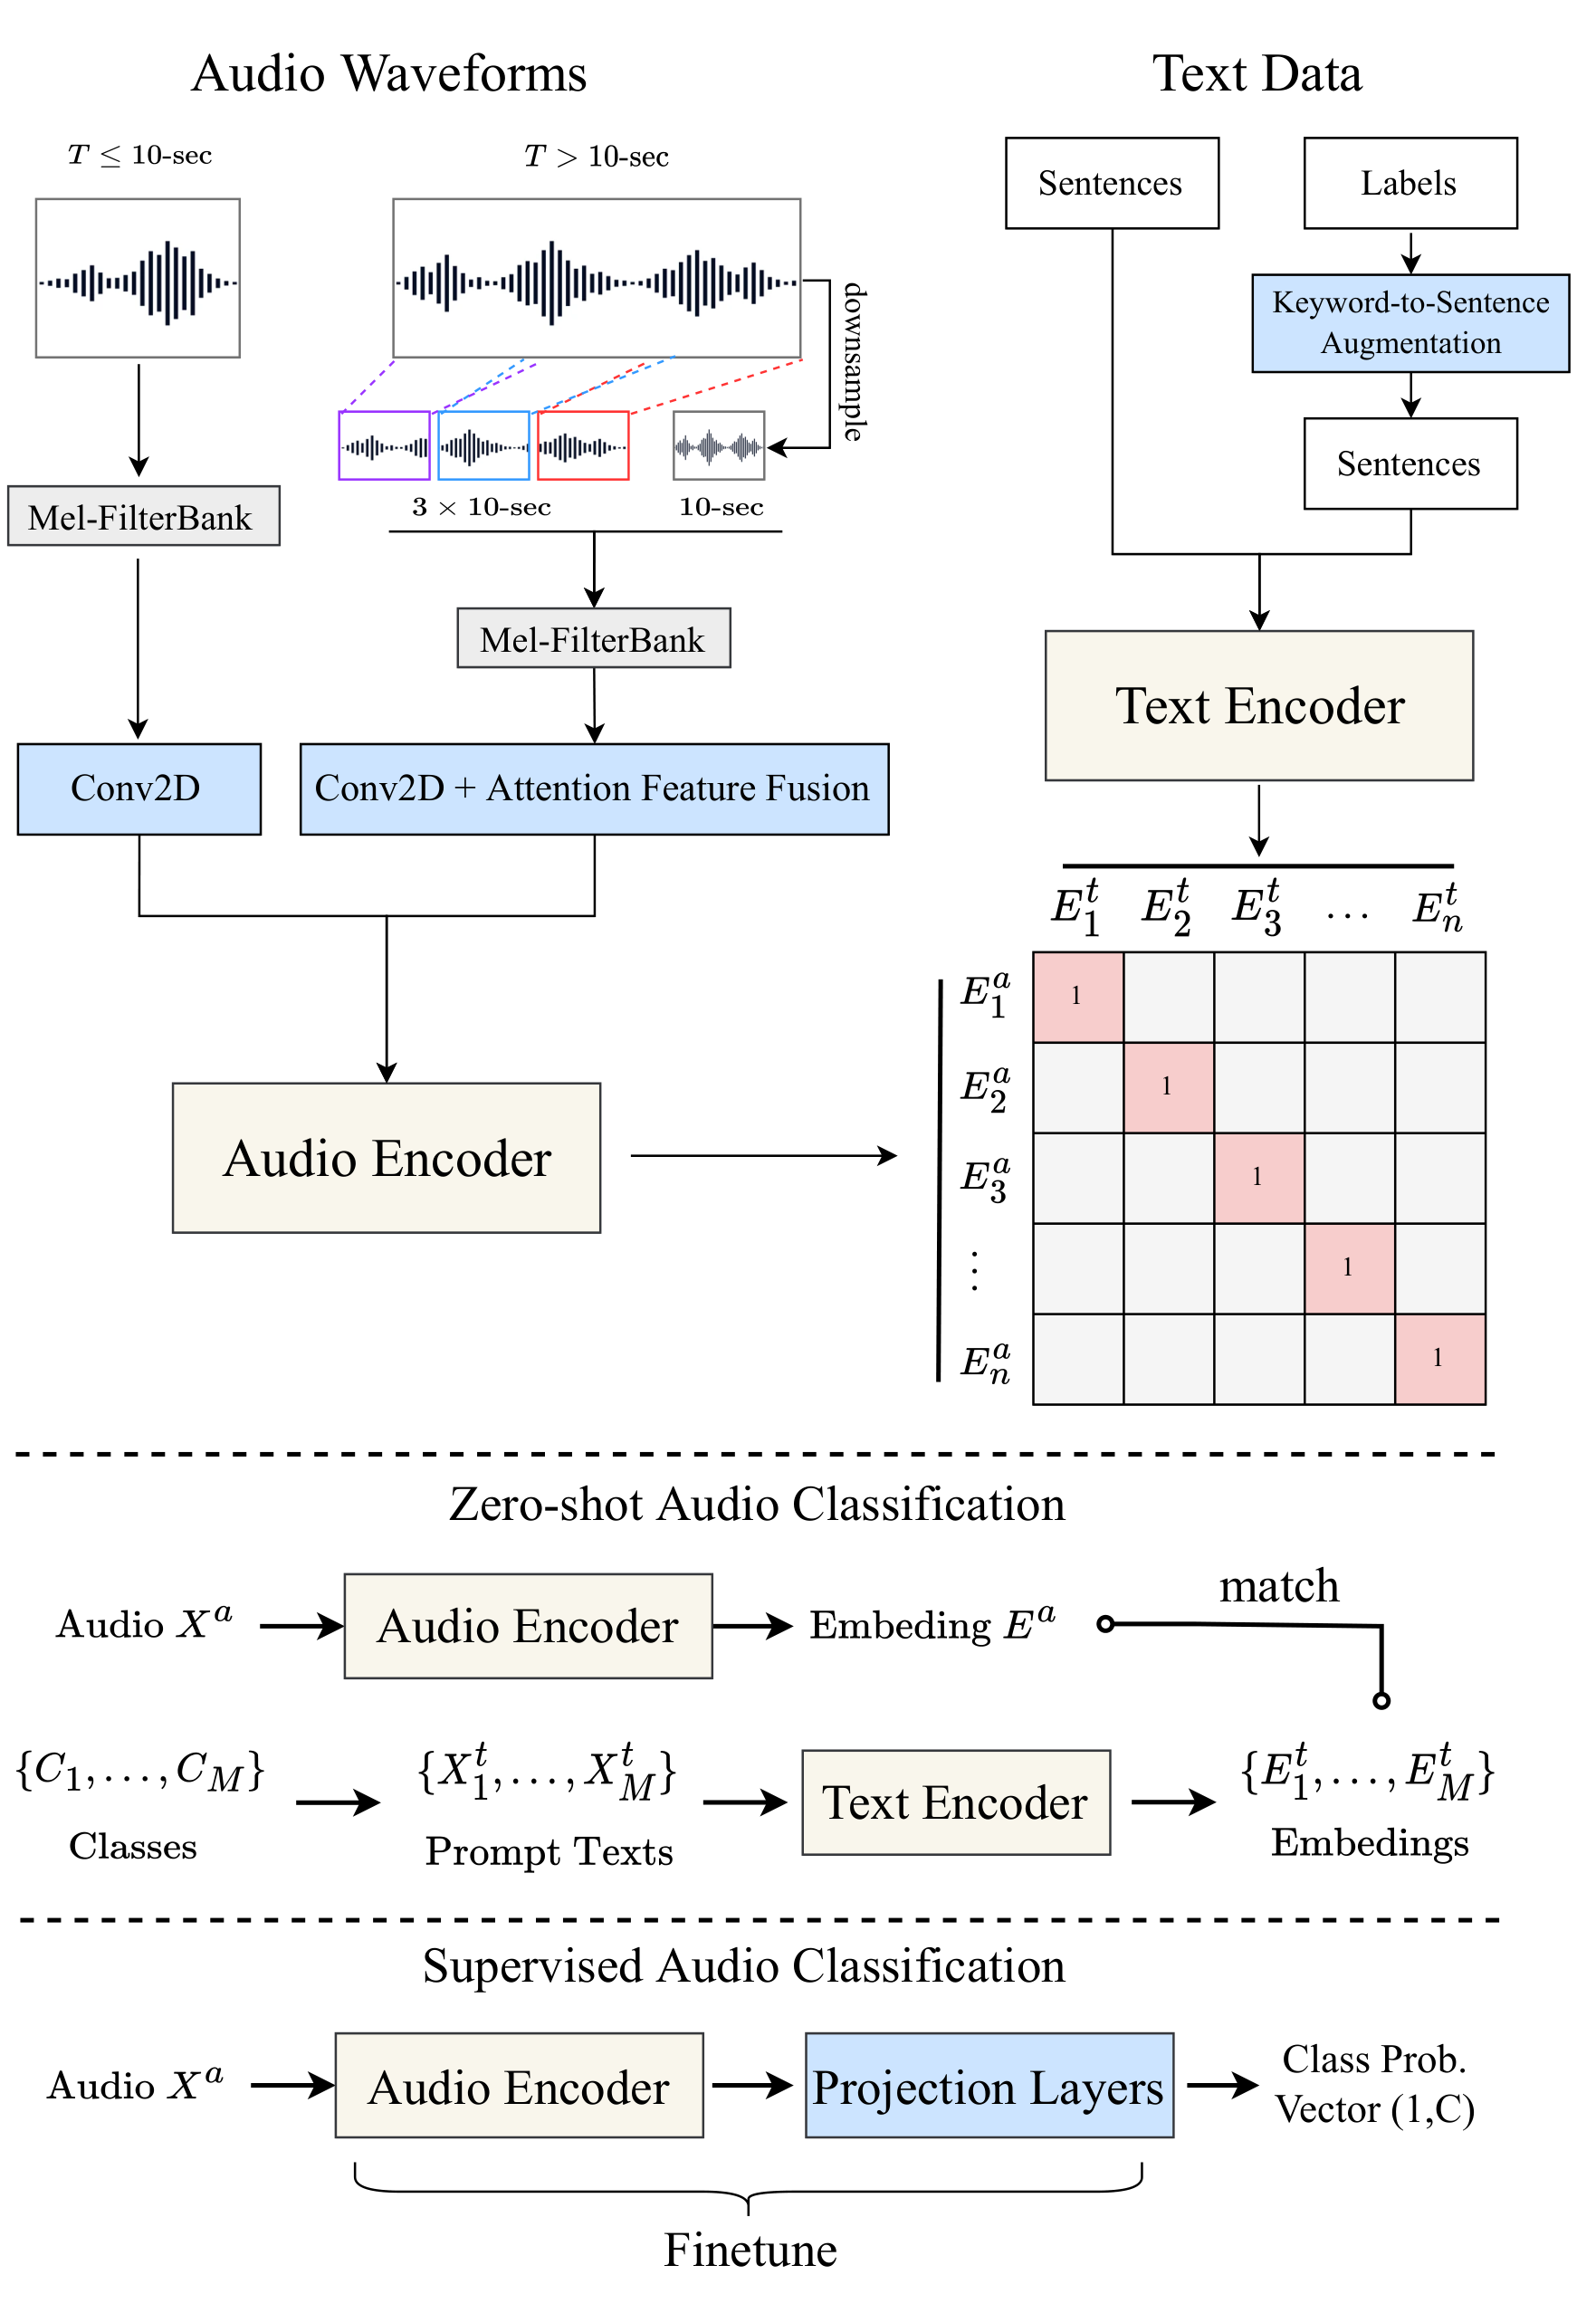
\includegraphics[width=0.6\textwidth]{Chapter4/audioclip-arch.png}
    \caption{CLAP model architecture used for embedding audio and text.}
    \label{fig:clap-model}
\end{figure}

\paragraph{CLAP: Multimodal Embedding Model}
CLAP is a transformer-based model trained to align audio and text modalities in a shared embedding space. It consists of two separate encoders:
\begin{itemize}
    \item \textbf{Audio Encoder:} Processes raw waveforms into feature embeddings using convolutional layers followed by transformers.
    \item \textbf{Text Encoder:} A transformer-based language model (similar to BERT) that embeds textual patient metadata.
\end{itemize}

The output of each encoder is a fixed-length vector, and CLAP is pretrained using contrastive learning to pull semantically aligned audio-text pairs closer in the embedding space.

\paragraph{Embedding Generation for Classification}
For this task:
\begin{itemize}
    \item Each breathing cycle was segmented from the audio and paired with patient text data.
    \item These inputs were passed through the CLAP model to generate audio and text embeddings.
    \item The embeddings were concatenated into a single feature vector.
    \item This fused embedding was used as input to a downstream neural classifier.
\end{itemize}

\paragraph{Classifier Architecture}
The classifier is a deep feedforward neural network with batch normalization, dropout regularization, and ReLU activations:
\begin{itemize}
    \item \textbf{Input:} Fused embedding vector of dimension $d$ (audio + text).
    \item \textbf{Layer 1:} Linear($d$, 512) $\rightarrow$ BatchNorm $\rightarrow$ ReLU $\rightarrow$ Dropout(0.5)
    \item \textbf{Layer 2:} Linear(512, 256) $\rightarrow$ BatchNorm $\rightarrow$ ReLU
    \item \textbf{Layer 3:} Linear(256, 64) $\rightarrow$ BatchNorm $\rightarrow$ ReLU
    \item \textbf{Output:} Linear(64, 3) $\rightarrow$ Softmax over respiratory classes (normal, crackles, wheezes)
\end{itemize}

\paragraph{Training Procedure}
\begin{itemize}
    \item \textbf{Loss Function:} Cross-entropy loss for multi-class classification.
    \item \textbf{Optimizer:} AdamW with initial learning rate of $1 \times 10^{-3}$ and weight decay of $1 \times 10^{-3}$.
    \item \textbf{Learning Rate Scheduler:} CosineAnnealingLR with $T_{\text{max}} = 10$.
    \item \textbf{Epochs:} Trained for 100 epochs with early stopping based on validation loss.
    \item \textbf{Batch Size:} Mini-batches of 32 samples for efficient GPU usage.
    \item \textbf{Fine-tuning Strategy:} CLAP weights were frozen during classifier training to preserve pretrained semantics and reduce training time.
\end{itemize}

\paragraph{Model Variants and Experiments}
Different modeling choices were explored to optimize performance:
\begin{itemize}
    \item \textbf{Fusion Strategy:} Simple concatenation of audio and text embeddings.
    \item \textbf{Embedding Size:} Tested with different encoder output dimensions.
    \item \textbf{Depth and Width of Classifier:} Adjusting hidden layer sizes and number of layers.
    \item \textbf{Freezing vs. Fine-tuning CLAP:} Partial fine-tuning yielded marginal improvements but increased training time.
\end{itemize}

\paragraph{Summary}
The modeling pipeline effectively combines audio and textual modalities through CLAP embeddings. A deep, regularized classifier leverages these representations for accurate respiratory sound classification. This architecture strikes a balance between expressiveness and efficiency, supporting real-time inference and deployment on modest hardware.

\break
\section{Evaluation}

\subsection*{Overview}
The model was evaluated on a held-out test set of 1,732 breathing cycles. Each sample included a fused CLAP embedding of audio and patient metadata. The classification targets were \texttt{normal}, \texttt{crackles}, and \texttt{wheezes}.

\begin{figure}[htbp]
    \centering
    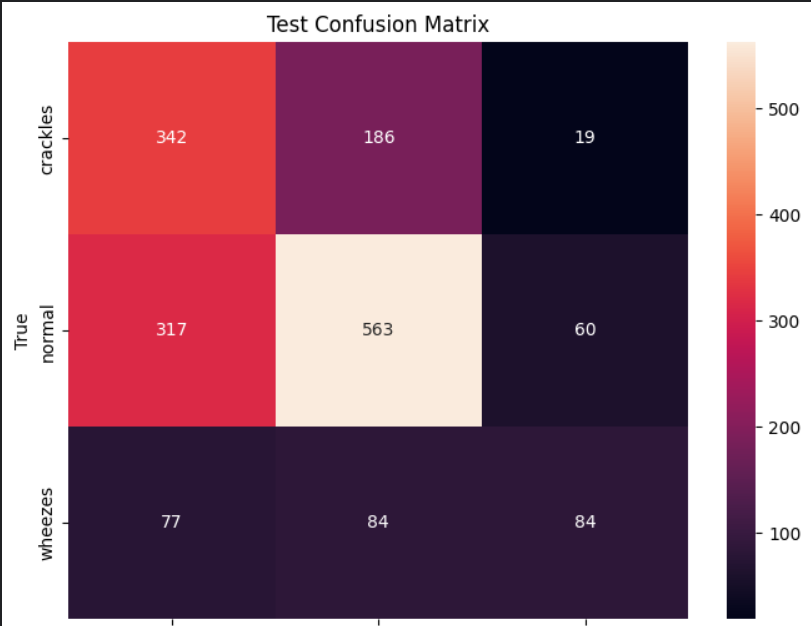
\includegraphics[width=0.7\linewidth]{Chapter4/pic.png}
    \caption{Test confusion matrix for respiratory sound classification.}
    \label{fig:confusion-matrix}
\end{figure}

\subsection{Performance Metrics}
\begin{itemize}
    \item \textbf{Accuracy:} 57.10\%
    \item \textbf{Macro F1-score:} 0.53
    \item \textbf{Weighted F1-score:} 0.57
    \item \textbf{Macro Precision:} 0.55
    \item \textbf{Macro Recall:} 0.52
\end{itemize}

\begin{table}[htbp]
\centering
\begin{tabular}{|l|c|c|c|c|}
\hline
\textbf{Class} & \textbf{Precision} & \textbf{Recall (Sensitivity)} & \textbf{F1-score} & \textbf{Support} \\
\hline
Crackles & 0.46 & 0.63 & 0.53 & 547 \\
Normal   & 0.68 & 0.60 & 0.64 & 940 \\
Wheezes  & 0.52 & 0.34 & 0.41 & 245 \\
\hline
\end{tabular}
\caption{Class-wise classification report.}
\end{table}

\subsection{Sensitivity and Specificity}
\begin{itemize}
    \item \textbf{Sensitivity (Recall):}
    \begin{itemize}
        \item Crackles: 0.625
        \item Normal: 0.599
        \item Wheezes: 0.343
        \item \textbf{Average:} 0.392
    \end{itemize}
    
    \item \textbf{Specificity:}
    \begin{itemize}
        \item Crackles: 0.668
        \item Normal: 0.659
        \item Wheezes: 0.947
        \item \textbf{Average:} 0.568
    \end{itemize}
\end{itemize}

\subsection{Observations}
\begin{itemize}
    \item The model performs best on the \texttt{normal} class, with an F1-score of 0.64.
    \item \texttt{Wheezes} are the hardest to classify (F1-score: 0.41), due to fewer examples and overlapping acoustic patterns with crackles.
    \item Specificity is highest for the \texttt{wheezes} class, indicating few false positives.
\end{itemize}

\subsection*{Summary}
The CLAP-based classifier shows promising overall accuracy and solid recall for crackles and normal sounds. Its lower sensitivity for wheezes suggests room for improvement through better balancing, augmentation, or fine-tuning the audio encoder. Still, the model maintains interpretability and scalability, aligning with the clinical goals of the system.

\section{Deployment (Model Serving)}

\paragraph{4.6.1 Overview\\}
To enable real-time inference, the trained multimodal CLAP-based classifier was deployed using a FastAPI web server. This server exposes a RESTful endpoint allowing users to upload a WAV audio file along with a patient information file in PDF format. The server extracts text from the PDF and combines it with the audio input to produce a diagnostic prediction.

\paragraph{4.6.2 File Structure\\}
The deployment folder contains the following core components:

\begin{itemize}
    \item \texttt{main.py} – FastAPI application containing preprocessing, inference, and routing logic.
    \item \texttt{model.pt} – Trained PyTorch classifier model weights.
    \item \texttt{label\_encoder.pkl} – Serialized \texttt{LabelEncoder} used to decode class indices into labels.
    \item \texttt{requirements.txt} – Specifies required Python libraries including \texttt{torch}, \texttt{transformers}, \texttt{PyMuPDF}, and \texttt{fastapi}.
    \item \texttt{Dockerfile} – Enables containerization of the app for consistent and scalable deployment.
\end{itemize}

\paragraph{4.6.3 API Endpoints\\}
Two endpoints are exposed:
\begin{itemize}
    \item \texttt{GET /} – Basic health check returning a simple greeting.
    \item \texttt{POST /predict} – Accepts:
    \begin{itemize}
        \item A WAV audio file.
        \item A PDF file containing patient information (e.g., age, sex, symptoms).
    \end{itemize}
    and returns a JSON response containing the predicted diagnostic label.
\end{itemize}

\paragraph{4.6.4 Processing Pipeline\\}
Upon receiving a request:
\begin{enumerate}
    \item The audio file is validated, loaded, resampled to 48\,kHz, converted to mono, and trimmed to a maximum of 8 seconds.
    \item The PDF file is parsed using \texttt{PyMuPDF} (\texttt{fitz}) to extract text-based metadata (e.g., "Patient is Male 36 , with BMI...").
    \item Audio and extracted text are processed using the CLAP processor to generate embeddings.
    \item Embeddings are passed to the trained classifier to generate class probabilities.
    \item The most probable class is decoded using \texttt{LabelEncoder} and returned.
\end{enumerate}

\paragraph{4.6.5 Robustness and Error Handling\\}
The API includes robust validation and fallback strategies:
\begin{itemize}
    \item Rejects non-WAV or non-PDF inputs.
    \item Handles corrupted or overly long audio clips.
    \item Gracefully processes empty or unreadable PDFs.
    \item Returns descriptive error messages and HTTP status codes for all edge cases.
\end{itemize}

\section*{4.7 Conclusion}
This section outlined the full CRISP-DM pipeline used to develop a multimodal respiratory sound classifier. By combining lung audio with patient metadata extracted from PDFs, the system leveraged CLAP embeddings for accurate, context-aware predictions. The final model was deployed using FastAPI, enabling real-time and scalable inference suitable for clinical settings.

\end{document}
